%%%%%%%%%%%%%%%%%%%%%%%%%%%%%%%%%%%%%%%%%%%%%%%%%%%%%%%%%%%%%%%%%%%
% Chapter2: Related Work
%%%%%%%%%%%%%%%%%%%%%%%%%%%%%%%%%%%%%%%%%%%%%%%%%%%%%%%%%%%%%%%%%%%

\chapter{Related Works}
\label{chap:related_work}

In this chapter, we analyze several approaches in handling time-series data, indicating the advantages and disadvantages of each approach. The related studies range from old methods such as ensemble model, deep feature-based approach, to recent methods which aim to decompose the input signal to frequency bands.

\section{Ensemble models}

% Phương sai trên time-series data là không cố định và thường thay đổi rất lớn qua các thời điểm. Sự thay đổi này thường được gọi là concept drift scenarios \cite{liu2025onsitnet}. Để tăng tính ổn định cho hệ thống dự đoán trong ngữ cảnh phương sai của dữ liệu biến thiên liên tục, thay vì sử dụng một mô hình, ensemble approach đề xuất sử dụng nhiều mô hình và kết hợp chúng lại để tạo ra các dự đoán.

The variance on time-series data is not constant and often varies greatly over time. This variation is often referred to as the concept of drift scenarios \cite{liu2025onsitnet}. To increase the stability of the prediction system in the context of continuously varying data variance, instead of using a single model, the ensemble approach proposes using multiple models and combining them to generate predictions.

% Thay vì huấn luyện một learner từ training data, ensemble methods huấn luyện một set of learners để giải quyết cùng một vấn đề. Dạng tổng quát của ensemble model $g(\mathbf{x})$ được thể hiện thông qua việc tổng hợp các mô hình $\{h_i, i=1\dots T\}$ như sau:

Instead of training a learner from training data, ensemble methods train a set of learners to solve the same problem. The general form of the ensemble model $g(\mathbf{x})$ is expressed by the aggregation of models $\{h_i, i=1\dots T\}$ as follows:

\begin{equation}
    g(\mathbf{x}) = \sum_{i=1}^T{\alpha_i h_i(\mathbf{x})} \text{, with } \sum_{i=1}^T{\alpha_i}=1
    \label{eq:ensemble}
\end{equation}

% Trong phương trình \ref{eq:ensemble} phép tính tổng được đề cập một cách trừu tượng, ám chỉ quá trình tổng hợp. $h_i$ được gọi là base learner. Base learner có thể được tạo ra từ bất kỳ base learning algorithm nào (e.g., decision tree, neural network, etc.,). Hầu hết các ensemble methods sử dụng cùng một base learning algorithm với training data khác nhau để huấn luyện base learners. Điều này tạo ra các base learners cùng loại (i.e., các base learners đều là decision tree hoặc neural network, etc.,).

In equation \ref{eq:ensemble} the summation operation is mentioned abstractly, referring to the process of ensemble. $h_i$ is called the base learner. The base learner can be created from any base learning algorithm (e.g., decision tree, neural network, etc.,). Most ensemble methods use the same base learning algorithm with different training data to train the base learners. This results in base learners of the same type (i.e., the base learners are all decision trees or neural networks, etc.,).

% Khả năng tổng quát hóa của ensemble model thường tốt hơn các base learners vì chúng có kết hợp các weak learners, vốn chỉ có thể dự đoán tốt hơn mức ngẫu nhiên một chút, thành một strong learners, có khả năng dự đoán với độ chính xác tốt hơn nhiều lần. Do đó, base learners thường được gọi là weak learners. Thật vậy, đối với mức noise tăng cần trong dữ liệu, sự kết hợp các mô hình luôn cho dự đoán tốt hơn so với việc sử dụng một mô hình đơn lẻ để dự đoán.

Ensemble models are often better at generalizing than base learners because they combine weak learners, which can predict only slightly better than random, to built a strong learner, which can predict with much better accuracy. Hence, base learners are often called weak learners. Indeed, when increasing levels of noise in the data, ensemble models always give better predictions than a single model.

% Ngoài ra, chi phí tính toán cho quá trình tạo ra nhiều base learners và kết hợp chúng không quá lớn so với việc xây dựng một single model bởi vì khi tạo ra một single model, chúng ta thường phải tạo ra rất nhiều phiên bản của mô hình đó trong quá trình tuning. Việc này tương đương với việc tạo ra nhiều base learners trong ensemble approach. Quá trình kết hợp các đặc trưng của ensemble model thông thường không tốn quá nhiều chi phí vì chiến lược kết hợp được sử dụng thường rất đơn giản (e.g., voting, averaging).

In addition, the computational cost of creating multiple base learners and combining them is not too large compared to building a single model because when creating a single model, we often have to create many versions of that model during tuning. This is equivalent to generating multiple base learners in the ensemble approach. The process of combining features of an ensemble model is usually not too expensive because the combination strategy is usually very simple (e.g., voting, averaging).

% Dựa trên quá trình tạo ra các base learners, chúng tôi đề cập đến hai hướng tiếp cận chính các phương pháp ensemble: \verb|Bagging| and \verb|Boosting| model. Trong đó, \verb|Bagging| tạo ra các base learners một cách song song còn \verb|Boosting| tạo ra các base learners một cách tuần tự.

Based on the process of generating base learners, we refer to two main approaches to ensemble methods: \verb|Bagging| and \verb|Boosting| models. Where, \verb|Bagging| generates base learners in parallel while \verb|Boosting| generates base learners sequentially.

\subsection{Bagging model}

% Động lực chính của \verb|Bagging| dựa trên việc khai thác sự độc lập của từng base learner. \verb|Bagging| giả định rằng, độ lỗi của mô hình có thể được giảm đáng kể bằng việc kết hợp các base learners độc lập. Khác với các hình dung ban đầu, từ ``bagging'' dù ám chỉ việc chia dữ liệu thành các bag nhưng không xuất phát từ từ ``bag'' mà là viết tắt của từ ``Bootstrap AGGregatING''. Như được đề cập trong tên gọi, \verb|Bagging| bao gồm hai ý tưởng chính là ``bootstrap'' và ``aggregation''.

The main motivation of \verb|Bagging| is based on exploiting the independence of each base learner. \verb|Bagging| assumes that the model error can be significantly reduced by combining independent base learners. Contrary to the initial conception, the word ``bagging'', although referring to dividing data into bags, does not come from the word ``bag'' but is an abbreviation of the word ``Bootstrap AGGregatING''. As mentioned in the name, \verb|Bagging| consists of two main ideas: ``bootstrap'' and ``aggregation''.

% \verb|Bagging| sử dụng bootstrap distribution để tạo ra các base learners khác nhau. Nói cách khác, nó áp dụng kỹ thuật bootstrap sampling để thu được các mẫu và huấn luyện các base learners trên các mẫu riêng biệt. Cụ thể, cho trước $n$ điểm dữ liệu huấn luyện, các mẫu chứa $n$ điểm dữ liệu được tạo ra bằng cách sampling with replacement từ $n$ điểm dữ liệu ban đầu. Bằng cách lặp lại quá trình này $T$ lần, $T$ mẫu được tạo thành.

\verb|Bagging| uses bootstrap distribution to generate different datasets for training base learners. In other words, it applies bootstrap sampling technique to obtain samples and train base learners on separate samples. Specifically, given $n$ training data points, samples containing $n$ data points are generated by sampling with replacement from $n$ original data points. By repeating this process $T$ times, $T$ samples are generated.

% Trong quá trình tổng hợp, \verb|Bagging| sử dụng cơ chế voting cho bài toán phân lớp và averaging cho bài toán hồi quy để tổng hợp output từ các base learners. Cụ thể, một \verb|Bagging| model với $T$ base learners $\{h_i, i=1\dots T\}$ trong bài toán hồi quy sẽ dự đoán instance $\mathbf{x}$ như sau:

During the aggregation process, \verb|Bagging| uses voting for the classification problem and averaging for the regression problem to aggregate output from base learners. Specifically, a \verb|Bagging| model with $T$ base learners $\{h_i, i=1\dots T\}$ in the regression problem will predict instance $\mathbf{x}$ as follows:

\begin{equation}
    \hat{y} = \frac{1}{T}\sum_{i=1}^T{h_i(\mathbf{x})}
\end{equation}

\subsection{Boosting model}

% Ý tưởng của \verb|Boosting| đến từ việc cải thiện một cách tuần tự quá trình dự đoán của mô hình trên các dữ liệu mà trước đó nó đã dự đoán sai. Sự cải thiện này được thực hiện thông qua quá trình điểu chỉnh lại phân phối của tập dữ liệu. Chúng tôi sẽ trình bày một toy example để làm rõ ý tưởng này.

The idea of \verb|Boosting| comes from sequentially improving the model's prediction performance on data that it previously predicted incorrectly. This improvement is done by adjusting the distribution of the data set. We will present a toy example to illustrate this idea.

% Cho tập dữ liệu $\mathcal{D}$ được rút ra từ không gian $\mathcal{X}$. Không gian $\mathcal{X}$ bao gồm ba phần $\mathcal{X}_1, \mathcal{X}_2$ và $\mathcal{X}_3$ chiếm tỷ lệ đều nhau. Giả sử mô hình $h_1$ sau khi huấn luyện trên $\mathcal{D}$ có thể dự đoán tốt các mẫu dữ liệu thuộc $\mathcal{X}_1, \mathcal{X}_2$ và có hiệu suất kém trên các mẫu dữ liệu thuộc $\mathcal{X}_3$. Lúc này, chúng ta có thể chỉnh sửa lỗi sai của $h_1$ bằng cách huấn luyện một mô hình $h_2$ trên tập dữ liệu $\mathcal{D}'$. Trong đó, $\mathcal{D}'$ là tập dữ liệu hiệu chỉnh từ $\mathcal{D}$ nhằm mục đích nhấn mạnh các mẫu $x\in\mathcal{X}_3$. Sau quá trình huấn luyện, $h_2$ có thể khắc phục được nhược điểm của $h_1$ trên không gian $\mathcal{X}_3$. Bằng việc kết hợp hai mô hình này, mô hình output được kỳ vọng là sẽ perform tốt trên cả ba sub-space của $\mathcal{X}$. Tuy nhiên, giả sử rằng, mô hình này chỉ perform tốt trên $\mathcal{X}_1, \mathcal{X}_3$. Lúc này, ta lại tiếp tục hiệu chỉnh tập dữ liệu huấn luyện để thu được $\mathcal{D}''$.

Given a data set $\mathcal{D}$ drawn from the space $\mathcal{X}$. The space $\mathcal{X}$ consists of three parts $\mathcal{X}_1, \mathcal{X}_2$ and $\mathcal{X}_3$ with equal proportions. Suppose that model $h_1$ after training on $\mathcal{D}$ can predict well on data samples belonging to $\mathcal{X}_1, \mathcal{X}_2$ and has poor performance on data samples belonging to $\mathcal{X}_3$. At this point, we can correct the error of $h_1$ by training a model $h_2$ on the data set $\mathcal{D}'$. In which, $\mathcal{D}'$ is the calibrated dataset from $\mathcal{D}$ to emphasize the samples $x\in\mathcal{X}_3$. After training, $h_2$ can overcome the weakness of $h_1$ on the space $\mathcal{X}_3$. By combining these two models, the output model is expected to perform well on all three sub-spaces of $\mathcal{X}$. However, suppose that this model only performs well on $\mathcal{X}_1, \mathcal{X}_3$. At this point, we continue to calibrate the training dataset to obtain $\mathcal{D}''$.

% Tóm lại, \verb|Boosting| hoạt động bằng cách huấn luyện các base learners một cách tuần tự sau đó kết hợp chúng để dự đoán. Các learner sau tập trung cải thiện lỗi của các learner trước.

In a nutshell, \verb|Boosting| works by training base learners sequentially and then combining them to make predictions. Later learners focus on improving the errors of earlier learners.

% cơ chế tổng hợp cùi bắp
% Điểm hạn chế của các mô hình ensemble nằm ở quá trình tổng hợp các base learners. Quá trình này dựa trên hai cơ chế voting và averaging ứng với bài toán phân lớp và bài toán hồi quy. Không khó để nhận thấy rằng hai cơ chế này thực sự rất đơn giản và cứng nhắc. Điều đó khiến cho ensemble approach dù cải thiện được khả năng tổng quát hóa so với việc huấn luyện một single model nhưng khả năng tổng quá hóa này thực sự chưa cao.

The limitation of ensemble models lies in the process of synthesizing base learners. This process is based on two mechanisms: voting and averaging, corresponding to the classification problem and the regression problem. \textbf{It is not difficult to see that these two mechanisms are really simple and rigid. That makes the ensemble approach, although improving the generalization ability compared to training a single model, the generalization ability is not really high.}

\section{Deep feature-based approach}

% không có cơ chế tổng hợp multiple source

\subsection{Convolutional neural network}

% phép tính convolution
% Điểm khởi đầu của Convolution neural network (\verb|CNN|) bắt nguồn từ convolution operation. Do đó, khi nói về \verb|CNN|, không thể không nhắc đến convolution operation. Giả sử chúng ta sử dụng một nguồn thu phát sóng để định vị một vật thể đang chuyển động. Thiết bị thu phát sóng này trả về một giá trị duy nhất $x(t)$, thể hiện vị trí của vật thể tại thời điểm $t$. Chúng ta có thể truy xuất vị trí này tại mọi thời điểm. Không may, giá trị trả về của thiết bị của chúng ta không thực sự chính xác mà bị nhiễu. Do đó, để thu được kết quả chính xác hơn tại một thời điểm $t$, chúng ta phải tổng hợp $x(t)$ và giá trị trước đó của nó: $x(a), a=t-1, t-2, etc.$ Trên thực tế, các thời điểm $a$ càng gần $t$ thì càng ảnh hưởng đến $x(t)$. Do đó, một weighting function được required để đánh trọng số cho các giá trị $x(a)$. Lúc này, giá trị ước lượng vị trí của vật tại thời điểm $t$ được tính bằng hàm $s(t)$ như sau:

The starting point of Convolution neural network (\verb|CNN|) is originated from convolution operation. Therefore, when talking about \verb|CNN|, it is impossible not to mention convolution operation. Suppose we use a sensor to locate a moving object. This sensor returns a single value $x(t)$, representing the position of the object at time $t$. We can retrieve this position at any time. Unfortunately, the returned value of our device is not really accurate but noisy. Therefore, to obtain a more accurate result at a time $t$, we have to aggregate $x(t)$ and its previous values: $x(a), a=t-1, t-2, etc.$ In fact, the closer $a$ is to $t$, the more it affects $x(t)$. Therefore, a weighting function is required to weight the values of $x(a)$. Now, the estimated value of the object's position at time $t$ is calculated using the function $s(t)$ as follows:

\begin{align}
    s(t) &= \int_{a=-\infty}^\infty{x(a) w(t-a) da}\\
    &= (x*w)(t)
\end{align}

% Phép tính trên được gọi là \textit{convolution} operation. Trên miền rời rạc, convolution operation hoạt động như sau:

The above operation is called \textit{convolution} operation. In discrete domains, the convolution operation works as follows:

\begin{align}
    (x*w)(t) = \sum_{a=-\infty}^\infty{x(a) w(t-a)}
\end{align}

% viết về conv1d, 2d, 3d...
% Điểm mấu chốt của phép tính này là chỉ ra một quan hệ cục bộ giữa đối tượng đang xét ($x(t)$) và các đối tượng $x(a)$ với $a$ gần $t$. Lấy cảm hứng từ điều này, nghiên cứu \cite{lecun1989handwritten} đề xuất mạng \verb|CNN|, sử dụng hai thành tố input (ứng với $x$) và kernel (ứng với $w$) và \textit{cross-correlation} operation thay vì convolution operation truyền thống. Tuy nhiên, \cite{lecun1989handwritten} vẫn gọi nó là convolution neural network. Về cơ bản, cross-correlation operation nhìn khá giống convolution operation ngoại trừ một sự thay đổi nhỏ trong index của input và kernel để thuật tiện cho việc cài đặt. Cụ thể, cross-correlation operation hoạt động như sau:

The key point of this operation is to show a local relationship between the object under consideration ($x(t)$) and the objects $x(a)$ with $a$ near $t$. Inspired by this, the research \cite{lecun1989handwritten} proposed a \verb|CNN| network, using two components input (corresponding to $x$) and kernel (corresponding to $w$) and \textit{cross-correlation} operation instead of the traditional convolution operation. However, \cite{lecun1989handwritten} still calls it a convolution neural network. Basically, the cross-correlation operation looks quite similar to the convolution operation except for a small change in the index of the input and kernel for convenience in implementation. Specifically, the cross-correlation operation works as follows:

\begin{align}
    (x*w)(t) = \sum_{a=-\infty}^\infty{x(t+a) w(a)}
\end{align}

% Điều đáng chú ý là \verb|CNN| không tổng hợp thông tin theo một chiều (trong ví dụ của chúng ta là chiều thời gian), mà còn có thể tổng hợp thông tin theo hai chiều (đối với ảnh RGB hoặc gray scale thông thường) hoặc ba chiều (đối với ảnh quang phổ bao gồm nhiều ảnh chụp đơn xếp chồng lên nhau). Tại đây, chúng tôi trình bày hai ứng dụng phổ biến của \verb|CNN| ứng với việc tổng hợp thông tin theo một chiều và hai chiều trên time-series data và dữ liệu dạng ảnh. Lưu ý rằng, các dữ liệu này có tính rời rạc, do đó, dấu tích phân trong phương trình gốc được thay bằng dấu tổng. Ngoài ra, do các thời điểm/vị trí càng xa sẽ ảnh hưởng càng ít đến thời điểm/vị trí đang xét, một giả định được sử dụng thường xuyên trong \verb|CNN| là sử ảnh hưởng là hoàn toàn cục bộ. Nghĩa là kernel được sử dụng sẽ có các giá trị khác 0 trong tầm ảnh hưởng và bằng 0 ở ngoài tầm ảnh hưởng. Có thể hình dung đơn giản rằng kernel như một window trượt dọc theo chiều của dữ liệu để tổng hợp thông tin.

It is worth noting that \verb|CNN| can aggregate information not only in one dimension (in our example, the time dimension), but can also aggregate information in two dimensions (for conventional RGB or gray scale images) or three dimensions (for spectral images consisting of multiple single-shot images stacked on top of each other). Here, we present two common applications of \verb|CNN| for one-dimensional and two-dimensional aggregation on time-series data and image data. Note that these data are discrete, so the integral sign in the original equation is replaced by a summation sign. In addition, since farther away positions/timestamps have less influence on the current position/timestamp, a commonly used assumption in \verb|CNN| is that the influence is totally local. That is, the kernel has non-zero values within the influence range and zero values outside the influence range. It can be simply visualized the kernel as a window that slides along the direction of the data to synthesize information.

% Ký hiệu $I, K$ lần lượt là input và kernel. Đối với time-series data, kernel chỉ có thể trượt dọc theo chiều thời gian của dữ liệu nên convolution operation được ký hiệu là \verb|Conv1D|. Giả sử dữ liệu đang xét là close price của cổ phiếu theo ngày của một công ty, kernel $K$ quy định mức ảnh hưởng cục bộ trong 5 ngày. Tại ngày thứ $i$, đặc trưng $F(i)$ được tổng hợp như sau:

Denote $I, K$ as the input and kernel, respectively. For time-series data, the kernel can only slide along the time direction of the data, so the convolution operation is denoted as \verb|Conv1D|. Suppose the data under consideration is the daily close price of a company's stock, the kernel $K$ specifies the local influence over 5 days. At day $i$, the feature $F(i)$ is synthesized as follows:

\begin{align}
    F(i) = (I*K)(i) = \sum_{m=1}^5{I(i+m) K(m)}
\end{align}

% Đối với dữ liệu dạng ảnh thông thường, $K$ trở thành một ma trận quy định mức ảnh hưởng của các pixel cục bộ lên pixel đang xét và có thể trượt theo hai chiều từ trái sang phải và từ trên xuống dưới. Do đó, convolution operation được ký hiệu là \verb|Conv2D|. Giả sử mức ảnh hưởng này là một vùng hình chữ nhật kích thước $(M\times N)$, tại pixel $(i,j)$, đặc trưng $F(i,j)$ được tổng hợp như sau:

For normal image data, $K$ becomes a matrix that determines the influence of local pixels on the pixel under consideration and can be slid in both directions from left to right and from top to bottom. Therefore, the convolution operation is denoted as \verb|Conv2D|. Suppose this influence is a rectangular region of size $(M\times N)$, at pixel $(i,j)$, the feature $F(i,j)$ is synthesized as follows:

\begin{align}
    F(i,j) = (I*K)(i,j) = \sum_m^M\sum_n^N{I(i+m, j+n)K(m,n)}
\end{align}

% Trong quá trình huấn luyện, \verb|CNN| cố gắng học một mức ảnh hưởng hợp lý từ đó có thể rút trích hiệu quả các đặc trưng không gian, thời gian của dữ liệu đầu vào. Sự hiệu quả của \verb|CNN| đến từ hai ý tưởng chính. Thứ nhất, dựa trên giả định rằng các đối tượng cục bộ mang lại nhiều ý nghĩa hơn đối với đối tượng đang xét hơn các đối tượng toàn cục, \verb|CNN| thu nhỏ không gian tìm kiếm tham số của mình từ một tập các tham số tương tác toàn diện với tất cả input thành một tập các tham số chỉ tương tác với các đối tượng cục bộ (kernel) nhưng mang lại nhiều ý nghĩa hơn. Giả sử mạng neural có $m$ inputs và $n$ output. Bằng việc sử dụng kernel kích thước $k\ll m$, độ phức tạp thời gian trong quá trình tính toán giảm từ $\mathcal{O}(mn)$ xuống còn $\mathcal{O}(kn)$ nhưng lại tăng được hiệu quả của mạng. Thứ hai, trong quá trình học, \verb|CNN| chỉ sử dụng duy nhất một kernel. Điều này làm giảm chi phí lưu trữ từ $\mathcal{O}(mn)$ trong mạng neural truyền thống xuống còn $\mathcal{O}(k)$.

During training, \verb|CNN| attempts to learn a reasonable influence level to efficiently extract the spatial and temporal features of the input data. The effectiveness of \verb|CNN| comes from two main ideas. First, based on the assumption that local features are more meaningful to the object under consideration than global features, \verb|CNN| reduces its parameter search space from a set of parameters that interact comprehensively with all inputs to a set of parameters that interact only with local features (kernels) but are more meaningful. Suppose the neural network has $m$ inputs and $n$ outputs. By using a kernel of size $k\ll m$, the time complexity of the computation is reduced from $\mathcal{O}(mn)$ to $\mathcal{O}(kn)$ but the efficiency of the network is increased. Second, during learning, \verb|CNN| uses only one kernel. This reduces the space complexity from $\mathcal{O}(mn)$ in traditional neural networks to $\mathcal{O}(k)$.

% Tuy nhiên, đối với time-series data nói chung và aperiodic time-series data nói riêng, tính chất dữ liệu tại một thời điểm bất kỳ không chỉ phụ thuộc vào các thời điểm gần đó mà còn phụ thuộc rất nhiều vào các thời điểm dài hạn trong quá khứ. Do đó, \verb|CNN| chỉ được sử dụng như một phương pháp hỗ trợ rút trích đặc trưng trong quá trình giải quyết các bài toán trên dữ liệu time-series.

\textbf{However, for time-series data in general and aperiodic time-series data in particular, the data properties at any given time depend not only on recent times but also on long-term times in the past. Therefore, \Verb|CNN| is only used as a method to support feature extraction in the process of solving problems on time-series data.}

% trong TH tệ, có thể viết thêm luồng làm việc của CNN: CNN -> pooling -> CNN -> pooling -> flatten -> clf head

\subsection{Recurrent Neural Network}

Thay vì hoạt động trên một lướt pixel như \verb|CNN|, Recurrent neural network (\verb|RNN|) \cite{rumelhart1986learning} hoạt động trên một chuỗi các giá trị $\mathbf{x}^{(1)},\dots,\mathbf{x}^{(\tau)}$. So với mạng mạng \verb|FullyConnected|, \verb|RNN| có thể mở rộng số lượng datapoint trong một chuỗi đến vô hạn mà không cần tăng kích thước của mạng. Nói cách khác, \verb|RNN| có khả năng làm việc trên các chuỗi dài hiệu quả hơn nhiều so với mạng neural truyền thống.

Tương tự như \verb|CNN|, \verb|RNN| cũng sử dụng một kiến trúc mạng cho phép chia sẻ tham số. Tuy nhiên, \verb|CNN| chia sẻ tham số trong nội bộ của một mẫu dữ liệu (cùng một kernel hoạt động trên các vùng cục bộ của một mẫu dữ liệu). \verb|RNN| chia sẻ tham số bằng cách sử dụng cùng một bộ tham số cho các mẫu dữ liệu khác nhau. Do đó, khi input một mẫu dữ liệu vào mô hình, output của mô hình chứa các thông tin của mẫu dữ liệu này và toàn bộ các mẫu dữ liệu trước đó. Điều này khiến cho việc mở rộng mô hình và apply mô hình lên các mẫu dữ liệu có độ dài khác nhau trở nên khả thi và hiệu quả hơn.

Cụ thể, gọi hàm $f$ là mạng \verb|RNN|. Hàm $f$ sử dụng bộ tham số $\theta$ để rút trích thông tin từ trạng thái $\mathbf{s}^{(t-1)}$ để tạo ra trạng thái $\mathbf{s}^{(t)}$:

\begin{align}
    \mathbf{s}^{(t)} = f\left( \mathbf{s}^{(t-1)}; \theta \right)
    \label{eq:recurrent}
\end{align}

Lưu ý rằng, $\mathbf{s}^{(t)}$ là một abstract variable, ám chỉ thông tin hiện tại phụ thuộc vào các thông tin trong quá khứ. Đối với chuỗi có độ dài $\tau$ bất kỳ, equation \ref{eq:recurrent} có thể được triển khai $\tau-1$ lần để nén các thông tin trong chuỗi vào các trạng thái $\mathbf{s}^{(t)}$.

Trong các mạng \verb|RNN| thông thường, biến trạng thái $\mathbf{s}$ được thể hiện bằng thông tin rút trích được từ mạng $\mathbf{h}$ và dữ liệu $\mathbf{x}$. Cụ thể, trạng thái hiện tại $\mathbf{h}^{(t)}$ được rút trích dựa trên trạng thái trước đó $\mathbf{h}^{(t-1)}$ (chứa thông tin về toàn bộ chuỗi trước đó) và mẫu dữ liệu hiện tại $\mathbf{x}^{(t)}$:

\begin{align}
    \mathbf{h}^{(t)} = f\left( \mathbf{h}^{(t-1)}, \mathbf{x}^{(t)}; \theta \right)
    \label{eq:rnn}
\end{align}

Phương trình \ref{eq:rnn} có thể được viết lại dưới dạng mô hình $g^{(t)}$ như sau:

\begin{align}
    \mathbf{h}^{(t)} = g^{(t)}\left( \mathbf{x}^{(t)}, \mathbf{x}^{(t-1)},\dots,\mathbf{x}^{(2)},\mathbf{x}^{(1)}; \theta \right)
    \label{eq:rnn_g}
\end{align}

Từ đây, có thể thấy rằng, mô hình $g$ không cần phải cập nhật tham số khi học từng mẫu $x^{(t)}$ như mạng neural truyền thống. Thay vào đó, nó có thể sử dụng thông tin từ một chuỗi $\mathbf{x}^{(1)},\dots,\mathbf{x}^{(\tau)}$ để cập nhật tham số thông qua mô hình $f$. Ngoài ra, việc sử dụng mô hình $f$ còn cải thiện khả năng tổng quát hóa của mô hình đối với những chuỗi có độ dài bất kỳ.

\begin{figure}[H]
    \centering
    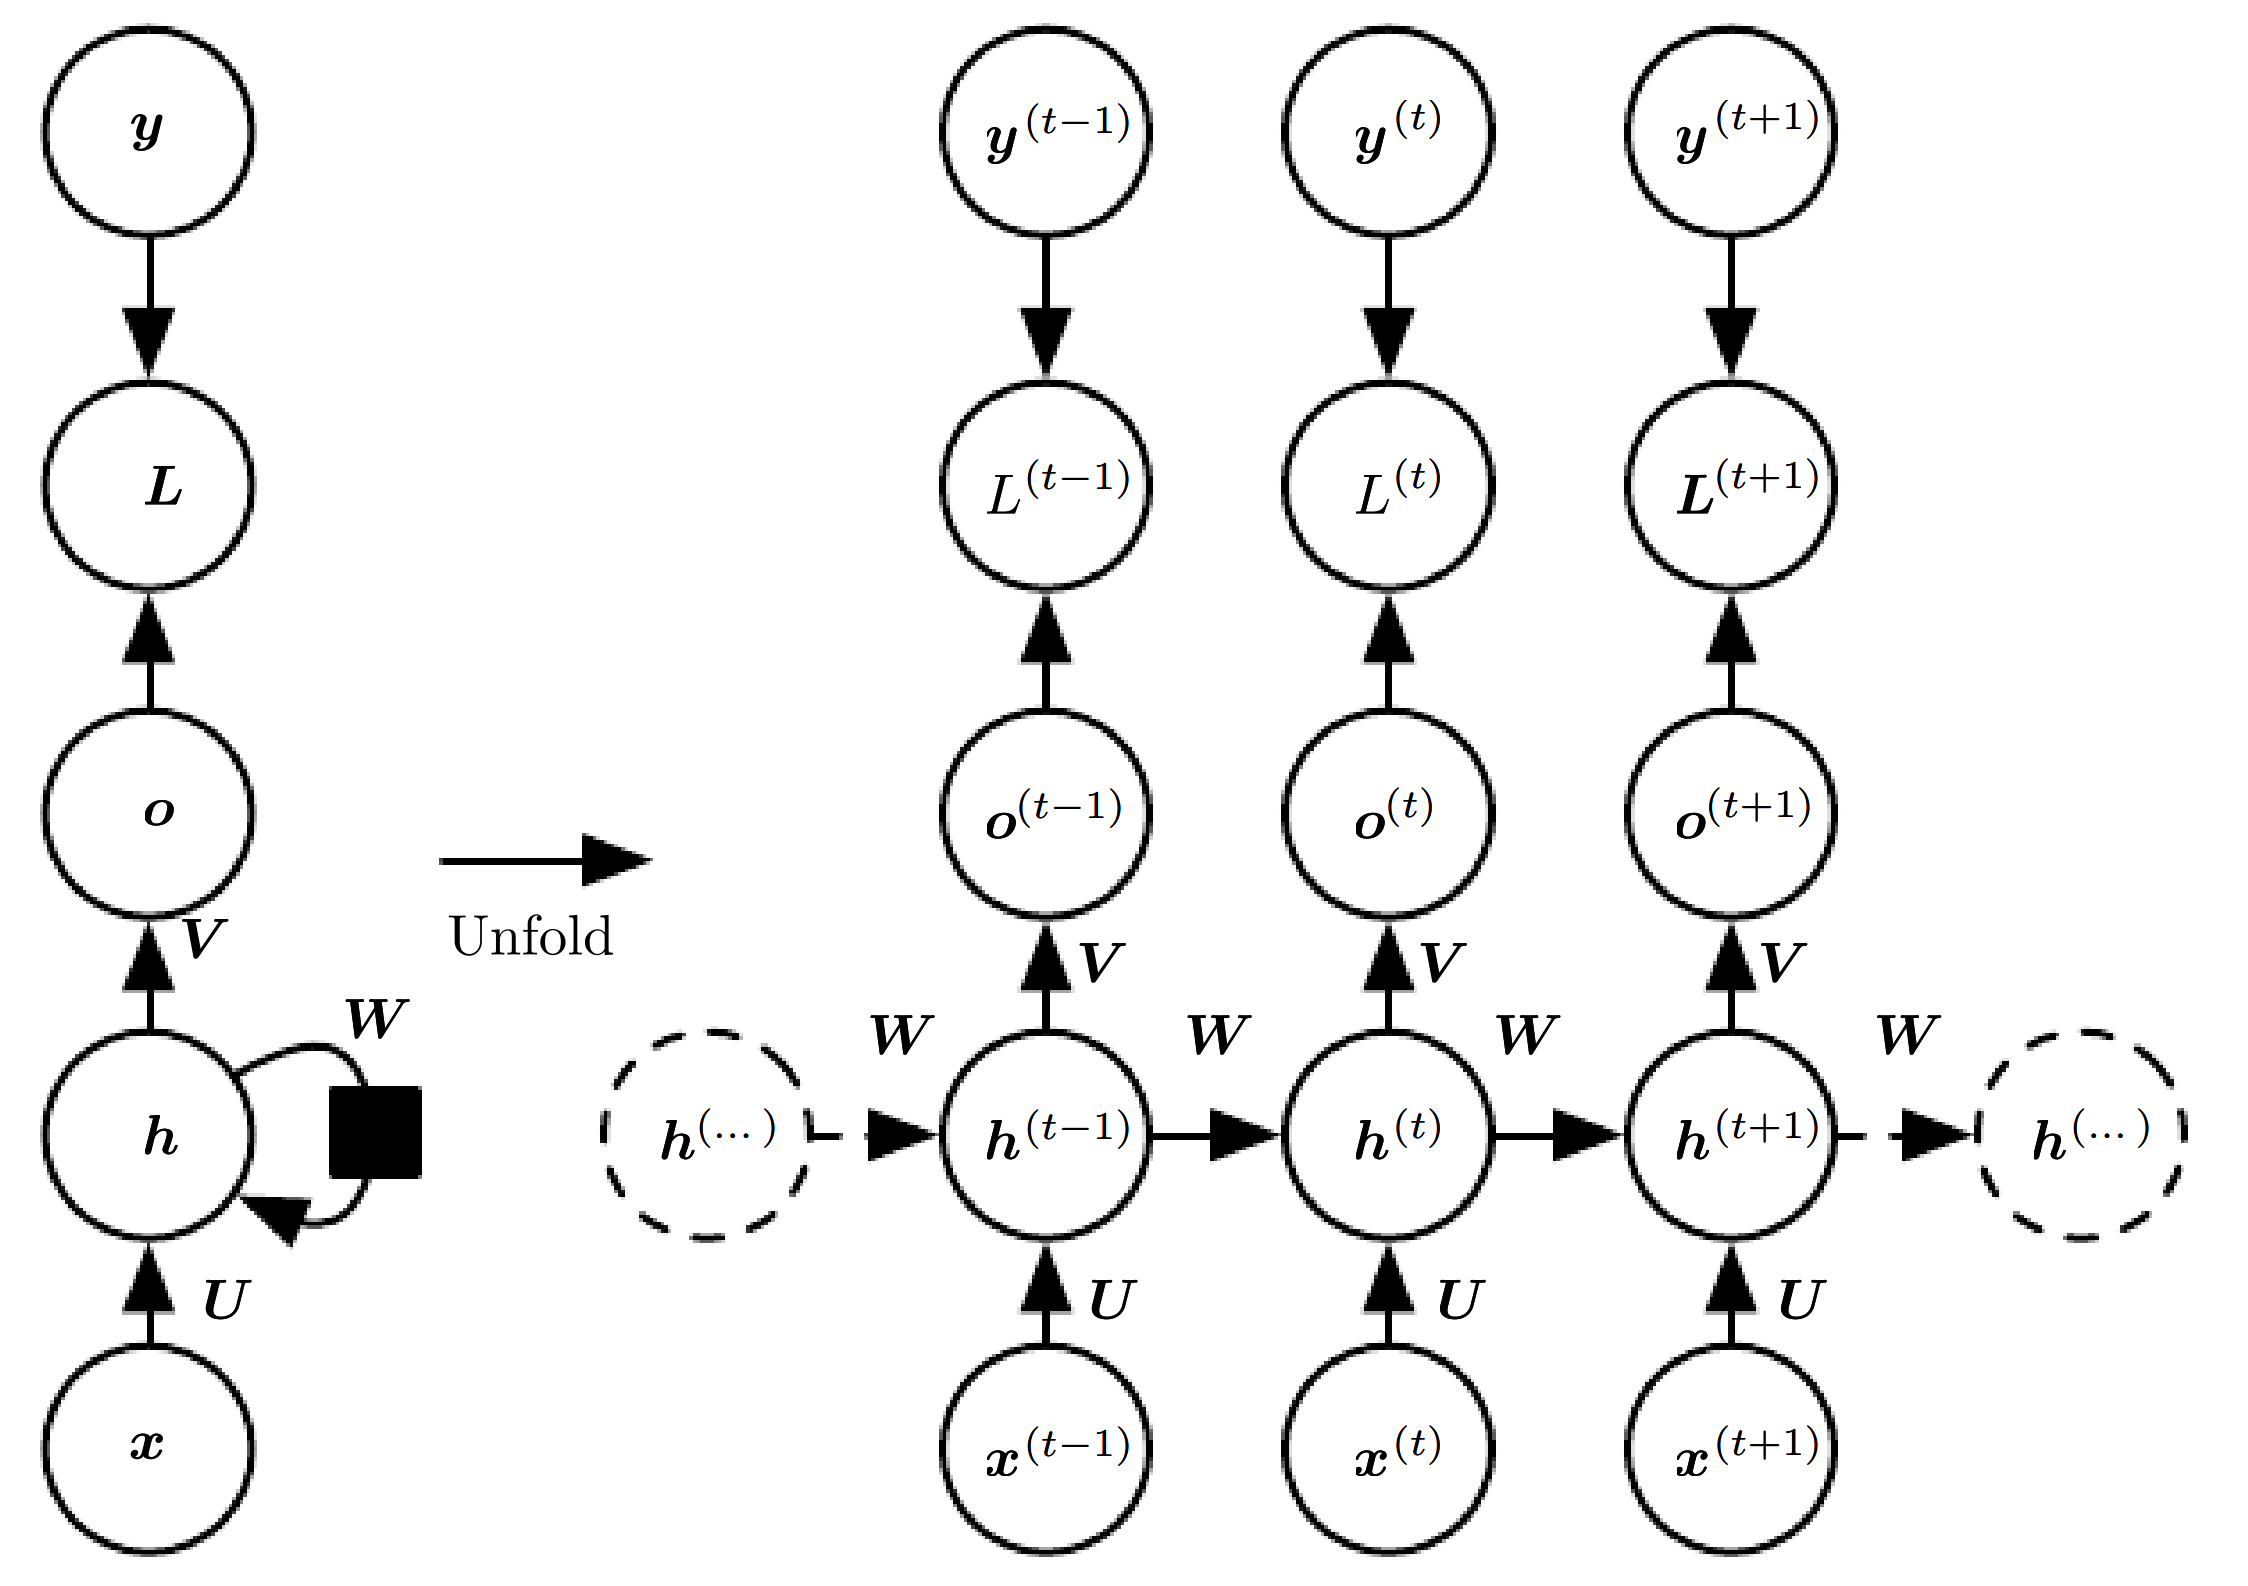
\includegraphics[width=\linewidth]{rnn.png}
    \cprotect\caption{The computational graph of \verb|RNN| in next-word prediction problem \cite{goodfellow2016deep}.}
    \label{fig:rnn}
\end{figure}

Dựa vào ý tưởng của recurrent function $f$ trình bày ở trên, chúng ta có thể thiết kế rất nhiều kiến trúc mạng \verb|RNN|. Tại đây, chúng tôi trình bày về một thiết kế đơn giản có đồ thị tính toán như hình \ref{fig:rnn}. Theo đó, mạng nhận vào một chuỗi các giá trị $\mathbf{x}$ với mục tiêu ánh xạ các giá trị này vào các đầu ra $\mathbf{o}$ khớp với $\mathbf{y}$. Để thực hiện điều này, mạng sử dụng ba bộ tham số chính: $\mathbf{U}$ để ánh xạ $\mathbf{x}$ vào không gian đặc trưng ẩn; $\mathbf{W}$ để ánh xạ đặc trưng ẩn của timestamp trước vào không gian đặc trưng ẩn của timestamp sau; $\mathbf{V}$ để ánh xạ đặc trưng ẩn vào không gian chứa các giá trị đầu ra chưa chuẩn hóa ($\mathbf{o}$). Giá trị dự đoán $\hat{y}$ sau đó được tính từ $\mathbf{o}$. Cả quá trình được thể hiện như sau:

\begin{align}
    \mathbf{a}^{(t)} &= \mathbf{b} + \mathbf{W}\mathbf{h}^{(t-1)} + \mathbf{U}\mathbf{x}^{(t)}\quad \text{($\mathbf{b}$ is bias vector)}\\
    \mathbf{h}^{(t)} &= \tanh\left( \mathbf{a}^{(t)} \right)\\
    \mathbf{o}^{(t)} &= \mathbf{c} + \mathbf{V}\mathbf{h}^{(t)}\quad \text{($\mathbf{c}$ is bias vector)}\\
    \hat{y}^{(t)} &= \text{softmax}\left( \mathbf{o}^{(t)} \right)
\end{align}

Độ lỗi của mô hình được tính bằng hàm \verb|CrossEntropyLoss| (equation \ref{eq:loss_rnn}). Hàm lỗi này được sử dụng để cập nhật các tham số của hàm $f$ thông qua kỹ thuật back-propagation through time.

\begin{align}
    L\left( \left\{ \hat{y}^{(t)} \right\}_{t=1}^\tau, \left\{ y^{(t)} \right\}_{t=1}^\tau \right) = \sum_{t=1}^\tau{L^{(t)}\left( \hat{y}^{(t)}, y^{(t)} \right)}
    \label{eq:loss_rnn}
\end{align}

Trong quá trình forward và backward, các bước tính toán được thực hiện tuần tự vì phải tuân theo trình tự thời gian. Do đó, time complexity của \verb|RNN| là $\mathcal{O}(\tau)$. Vì phải lưu trữ các giá trị đạo hàm sau để tính toán các giá trị đạo hàm trước đó (theo Chain rule), space complexity của thuật toán cũng là $\mathcal{O}(\tau)$. Do đó, đối với các chuỗi dài, chi phí tính toán có thể sẽ rất lớn.

\subsection{Long Short-Term Memory}

Khi làm việc trên các chuỗi dài, \verb|RNN| rất dễ mắc phải vấn đề \textit{vanishing gradient} hoặc \textit{exploding gradient}. Thật vậy, quá trình huấn luyện của \verb|RNN| đòi hỏi việc sử dụng Chain rule cho tất cả các trạng thái từ $t=\tau$ đến $t=1$. Quá trình này bao gồm rất nhiều phép nhân ma trận và vector. Do đó, nếu các phần tử trong ma trận hoặc vector đó nhỏ hơn 1, đạo hàm theo thời gian sẽ hội tụ về 0. Ngược lại, nếu các phần tử đó lớn hơn 1, theo thời gian, đạo hàm sẽ tiến đến vô cùng.

% viết 1 chút về bidirectional lstm

\section{Frequency decomposition approach}

% không có cơ chế tổng hợp multiple source

\subsection{A transformer-based method}

% require massive overhead

\subsection{NHITS}

% Neural Hierarchical Interpolation for Time Series Forecasting (\verb|NHITS|) \cite{challu2023nhits} được thiết kế để hướng đến việc dự đoán một long-horizon time-series data bằng cách phân rã tín hiệu đầu vào thành các dải tần số riêng biệt. Cấu trúc của \verb|NHITS| bao gồm $S$ stack, mỗi stack bao gồm $B$ block nối tiếp nhau. Tại mỗi block, một Multi-layer perceptron (\verb|MLP|) sử dụng dữ liệu lịch sử để dự đoán chính nó và dữ liệu tương lai (see figure \ref{fig:nhits}).

Neural Hierarchical Interpolation for Time Series Forecasting (\verb|NHITS|) \cite{challu2023nhits} is designed to target the prediction of long-horizon time-series data by decomposing the input signal into discrete frequency bands. The structure of \verb|NHITS| consists of $S$ stacks, each stack consisting of $B$ consecutive blocks. At each block, a Multi-layer perceptron (\verb|MLP|) uses historical data to predict itself and future data (see figure \ref{fig:nhits}).

\begin{figure}[H]
    \centering
    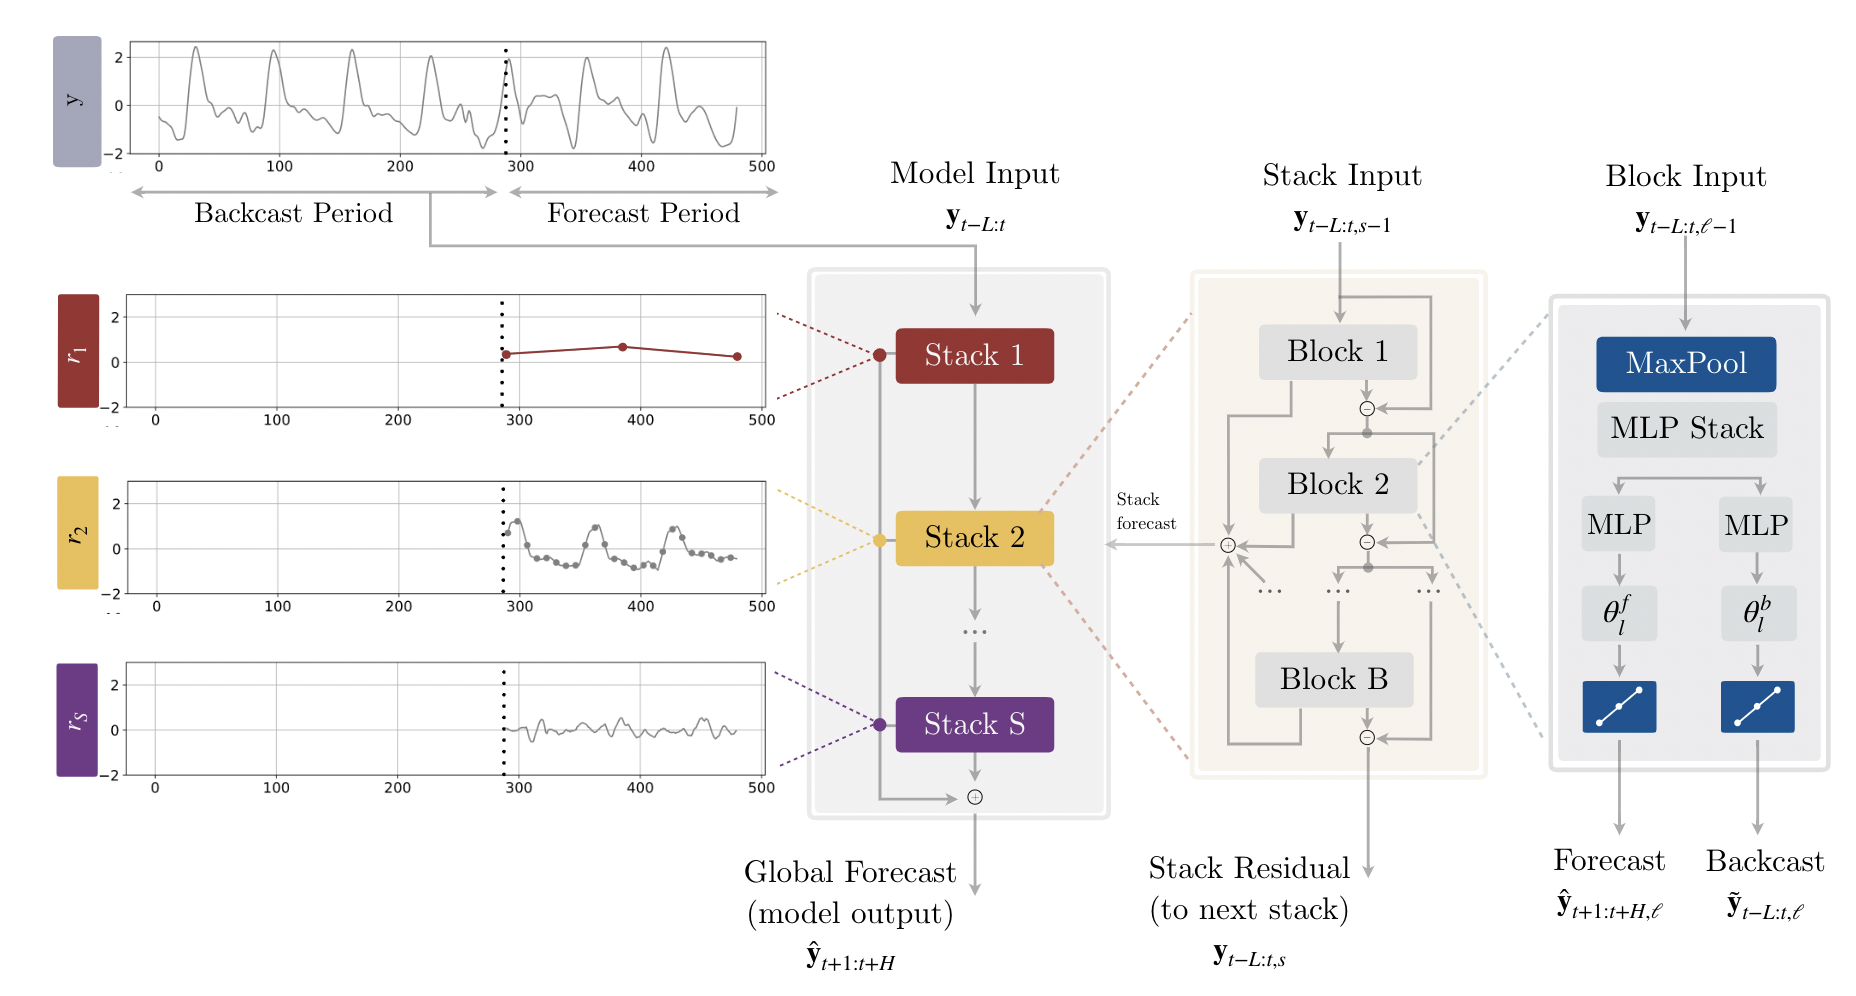
\includegraphics[width=\textwidth]{nhits-arch.png}
    \cprotect\caption{\verb|NHITS| architecture \cite{challu2023nhits}.}
    \label{fig:nhits}
\end{figure}

% Cụ thể, tại block $l$, với $L$ mẫu dữ liệu quá khứ ($\mathbf{y}_{t-L:t, l-1}$), một \verb|MLP| sẽ sử dụng lần lượt ba kỹ thuật Multi-rate signal sampling, Non-linear regression, và Hierarchical interpolation để hồi quy dữ liệu quá khứ và dự đoán dữ liệu tương lai.

Specifically, at block $l$, with $L$ historical samples ($\mathbf{y}_{t-L:t, l-1}$), an \verb|MLP| use three techniques, Multi-rate signal sampling, Non-linear regression, and Hierarchical interpolation, respectively, to regress past data and predict future data.

% \textbf{Multi-rate signal sampling}. \verb|MaxPool| layer với kernel size $l$ nén dữ liệu ban đầu vào $\mathbf{y}_{t-L:t, l}^{(p)}$ (equation \ref{eq:maxPool}). Khi $k_l$ lớn, lượng dữ liệu được xét trong một cửa sổ trượt lớn, mạng sẽ chú ý đến các sóng tín hiệu với bước sóng dài (tần số thấp). Khi $k_l$ nhỏ, các đặc trưng thu được là của các bước sóng nhỏ (tần số cao). Bằng việc sử dụng lớp \verb|MaxPool|, các \verb|MLP| sẽ có khả năng làm việc trên một dải tần nhất định, giúp tăng hiệu quả của việc phân rã tần số. Không chỉ dừng lại ở việc phân tách dải tần, \verb|MaxPool| về cơ bản làm giảm kích thước của tín hiệu đầu vào, giúp tiết kiệm bộ nhớ trong quá trình training và inference.

\textbf{Multi-rate signal sampling}. \verb|MaxPool| layer with kernel size $l$ compresses the original data into $\mathbf{y}_{t-L:t, l}^{(p)}$ (equation \ref{eq:maxPool}). When $k_l$ is large, the amount of data considered in a sliding window is also large, the network will pay more attention to input signal with long wavelengths (low frequencies). When $k_l$ is small, the obtained features are of short wavelengths (high frequencies). By using \verb|MaxPool| layer, \verb|MLP| will be able to work on a certain frequency band, which helps to increase the efficiency of frequency decomposition. Not only stopping at frequency band decomposition, \verb|MaxPool| essentially reduces the size of the input signal, helping to save memory during training and inference.

\begin{align}
    \mathbf{y}_{t-L:t, l}^{(p)} = \mathbf{MaxPool}\left( \mathbf{y}_{t-L:t, l-1}, k_l \right)
    \label{eq:maxPool}
\end{align}

% \textbf{Non-linear regression}. Sau khi nén dữ liệu, \verb|NHITS| tiến hành học các hệ số nội suy bằng các perceptron layer xếp chồng với hàm kích hoạt phi tuyến (\verb|FullyConnected|). Mục tiêu của \verb|FullyConnected| là tạo ra các vector $\mathbf{\theta}_l^f, \mathbf{\theta}_l^b$ (equation \ref{eq:non_linear}). Đây là hai vector nội suy forecast và backcast, được dùng để tổng hợp các giá trị đầu ra của block $l$ bằng hàm nội suy $g(\cdot)$. Trong đó, $\mathbf{\theta}_l^f$ được dùng để dự báo các giá trị tương lai còn $\mathbf{\theta}_l^b$ được dùng để hồi quy các giá trị input.

\textbf{Non-linear regression}. After compressing the data, \verb|NHITS| learns the interpolation coefficients using stacked perceptron layers with a nonlinear activation function (\verb|FullyConnected|). The goal of \verb|FullyConnected| is to generate the vectors $\mathbf{\theta}_l^f, \mathbf{\theta}_l^b$ (equation \ref{eq:non_linear}). These are the two interpolation vectors forecast and backcast, which are used to aggregate the output values of block $l$ using the interpolation function $g(\cdot)$. In which, $\mathbf{\theta}_l^f$ is used to forecast future values and $\mathbf{\theta}_l^b$ is used to regress the input values.

\begin{align}
    \mathbf{\theta}_l^b &= \mathbf{FullyConnected}^b \left( \mathbf{y}_{t-L:t, l}^{(p)} \right)\\
    \mathbf{\theta}_l^f &= \mathbf{FullyConnected}^f \left( \mathbf{y}_{t-L:t, l}^{(p)} \right)\\
    \label{eq:non_linear}
\end{align}

% \textbf{Hierarchical interpolation}. Để dự đoán $H$ giá trị tương lai, một mạng neural thông thường phải thiết kế lại số neuron đầu ra. Đôi với mô hình transformer, muốn tăng số mẫu đầu ra, cần phải tăng số mẫu đầu vào để các layer cross-attention hoạt động hiệu quả. Điều này khiến cho quá trình huấn luyện truyền thống tiêu tốn rất nhiều tài nguyên khi có nhu cầu dự đoán $H$ lớn. \verb|NHITS| giải quyết vấn đề này bằng cách sử dụng phương trình nội suy với các hệ số nội suy đã được chuẩn bị trước ở bước \textbf{Non-linear regression} (equation \ref{eq:interpolation}). Số chiều của các hệ số nội suy trong mỗi stack được quy định bởi expressiveness ratio $r_l$: $\left| \theta_l \right| =  \left \lceil r_l H \right \rceil$. Thông thường, expressiveness ratio sẽ rất nhỏ ở các stack đầu tiên và tăng dần về cuối. Theo đó, các stack có thể mô phỏng lại các tần số từ thấp đến cao. Ngoài ra, bằng việc sử dụng hàm nội suy, \verb|NHITS| không cần quá nhiều phần cứng để huấn luyện mạng neural trong trường hợp $H$ lớn.

\textbf{Hierarchical interpolation}. To forecast $H$ future values, a conventional neural network must redesign the number of output neurons. For transformer models, to increase the number of output samples, it is necessary to increase the number of input samples so that the cross-attention layers can work effectively. This makes the traditional training process very resource-consuming when there is a need to predict large $H$. \verb|NHITS| solves this problem by using an interpolation equation with pre-prepared interpolation coefficients in the \textbf{Non-linear regression} step (equation \ref{eq:interpolation}). The dimensionality of the interpolation coefficients in each stack is determined by the expressiveness ratio $r_l$: $\left| \theta_l \right| = \left \lceil r_l H \right \rceil$. Typically, the expressiveness ratio will be very small in the first stacks and gradually increase towards the end. Accordingly, the stacks can simulate frequencies from low to high. In addition, by using the interpolation function, \verb|NHITS| does not require too much hardware to train the neural network in the case of large $H$.

\begin{align}
    \mathbf{\hat{y}}_{t-L:t, l} &= g\left(\mathbf{\theta}_l^b\right)\\
    \mathbf{\hat{y}}_{t+1:t+H, l} &= g\left(\mathbf{\theta}_l^f\right)
    \label{eq:interpolation}
\end{align}

% Đầu ra của block $l$ là giá trị forecast $\mathbf{\hat{y}}_{t+1:t+H, l}$ và giá trị backcast $\mathbf{\hat{y}}_{t-L:t, l}$. Input of block $l+1$ is the difference between the its backcast and its output (\ref{eq:input_l1}).

The output of block $l$ is the forecast value $\mathbf{\hat{y}}_{t+1:t+H, l}$ and the backcast value $\mathbf{\hat{y}}_{ t-L:t, l}$. Input of block $l+1$ is the difference between its backcast and its output (\ref{eq:input_l1}).

\begin{align}
    \mathbf{y}_{t-L:t, l+1} = \mathbf{y}_{t-L:t, l-1} - \mathbf{\hat{y}}_{t-L:t, l}
    \label{eq:input_l1}
\end{align}

% Tổng hợp các giá trị forecast của $B$ block như phương trình \ref{eq:sum_block}, ta được giá trị forecast của một stack. Cuối cùng, tổng hợp giá trị forecast của các stack như phương trình \ref{eq:sum_stack}, ta được giá trị forecast dự đoán của toàn mạng.

Summing the forecast values of $B$ blocks as in equation \ref{eq:sum_block}, we get the forecast value of a stack. Finally, summing the forecast values of the stacks as in equation \ref{eq:sum_stack}, we get the predicted forecast value of the entire network.

\begin{align}
    \mathbf{\hat{y}}_{t+1:t+H}^s &= \sum_{l=1}^{B}{\mathbf{\hat{y}}_{t+1:t+H, l}} \label{eq:sum_block}\\
    \mathbf{\hat{y}}_{t+1:t+H} &= \sum_{s=1}^{S}{\mathbf{\hat{y}}_{t+1:t+H}^s} \label{eq:sum_stack}
\end{align}

% Bằng cách xếp chồng các stack, stack sau nhận vào phần dư của stack trước, kiến trúc trên được kỳ vọng là sẽ phân rã dữ liệu thành các frequency bands khác nhau (weekly, daily, even hourly). Trong thực tế, \verb|NHITS| perform rất tốt đối với các bộ dữ liệu có tính chu kỳ cao như mức tiêu thụ điện, thời tiết, giao thông. Tuy nhiên, chúng tôi đang hướng đến aperiodic time-series dataset, vốn có tính chu kỳ rất thấp. Điều này gây ra khó khăn rất lớn cho \verb|NHITS|.

By concatenating stacks, each receiving the remainder of the previous stack, \textbf{the above architecture is expected to decompose the data into different frequency bands (weekly, daily, even hourly)}. In practice, \verb|NHITS| performs very well for highly periodic datasets such as electricity consumption, weather, traffic. \textbf{However, we are aiming for an aperiodic time-series dataset, which has very low, or even non-existent, periodicity}. This poses a huge challenge for \verb|NHITS|.

\section{Optimization-based Meta-learning}
\label{sec:ml}

% Meta-learning (ML) là một phương pháp huấn luyện cho phép mô hình học có thể gia tăng kinh nghiệm qua việc thực hiện nhiều task khác nhau trong cùng một phân phối task. Việc này trạng bị cho mô hình học máy khả năng tổng quát hóa cao, thích ứng nhanh trên task mới chỉ sau một vài bước huấn luyện với dữ liệu huấn luyện giới hạn \cite{hospedales2021meta, vettoruzzo2024advances}. Với khả năng này, ML được sử dụng rất nhiều trong các tác vụ đòi hỏi khả năng đáp ứng của mô hình trên dữ liệu (e.g. cá nhân hóa mô hình học \cite{chen2018federated, fallah2020personalized,nguyen2022meta}, domain adaptation trong online learning \cite{hu2023meta, khoee2024domain}).

Meta-learning (ML) is a training method that allows a learning model to gain experience by performing many different tasks in the same task distribution. This equips the machine learning model with the ability to generalize highly and adapt quickly to new tasks after only a few training steps with limited training data \cite{hospedales2021meta, vettoruzzo2024advances}. With this ability, ML is widely used in tasks that require the ability to fast adapt to new data (e.g. personalization of learning models \cite{chen2018federated, fallah2020personalized,nguyen2022meta}, domain adaptation in online learning \cite{hu2023meta, khoe2024domain}).

% Đối với phương pháp huấn luyện mô hình học truyền thống, chúng ta huấn luyện mô hình dự đoán $\hat{y} = f_\theta(\mathbf{x})$ trên tập dữ liệu $\mathcal{D}_t = \left\{ \left(\mathbf{x}_i, y_i \right) \right\}$ của task $t$. Ký hiệu $\mathcal{L}$ là hàm lỗi, $\phi$ là prior knowledge, mục tiêu của quá trình huấn luyện là tối thiểu hóa hàm lỗi trên tập dữ liệu $\mathcal{D}$ bằng cách tìm tham số $\theta$ thỏa mãn:

For the traditional learning model training method, we train the prediction model $\hat{y} = f_\theta(\mathbf{x})$ on the dataset $\mathcal{D}_t = \left\{ \left(\mathbf{x}_i, y_i \right) \right\}$ of task $t$. Denote $\mathcal{L}$ is the error function, $\phi$ is the prior knowledge, the goal of the training process is to minimize the error function on the dataset $\mathcal{D}$ by finding the parameter $\theta$ that satisfies:

\begin{equation}
    \theta^* = \arg\min_{\theta}{\mathcal{L}(\mathcal{D}_t; \theta, \phi)}
\end{equation}

% Hướng tiếp cận của ML nằm ở chỗ cố gắng học một prior knowledge $\phi$ thật tốt. Điều này đạt được thông qua việc học một phân phối task $\mathcal{T}$ \cite{hospedales2021meta}. Sau khi học được một prior knowledge tốt, có thể sử dụng prior knowledge này cho các task mới trong cùng phân phối task $\mathcal{T}$. Về mặt toán học, ký hiệu $\mathcal{L}(\mathcal{D}_t, \phi)$ là hàm lỗi biểu diễn sự hiệu quả của việc sử dụng $\phi$ trong huấn luyện mô hình trên task $T$, mục tiêu của ML được biểu diễn như sau:

The ML approach is to try to learn a good prior knowledge $\phi$. This is achieved by learning a task distribution $\mathcal{T}$ \cite{hospedales2021meta}. Once a good prior knowledge is learned, it can be used for new tasks in the same task distribution $\mathcal{T}$. Mathematically, denote $\mathcal{L}(\mathcal{D}_t, \phi)$ is the error function that represents the effectiveness of using $\phi$ in training the model on task $T$, the ML goal is expressed as follows:

\begin{equation}
    \min_{\phi} \mathop{\mathbb{E}}_{t\sim \mathcal{T}} \mathcal{L}(\mathcal{D}_t, \phi)
\end{equation}

\subsection{Model-Agnostic Meta-Learning (MAML)}

% Đối với hướng tiếp cận dựa trên tối ưu, một thuật toán ML cơ bản, điển hình là \verb|MAML|, sẽ được học trên nhiều tác vụ $t$ rút ra từ cùng một phân phối tác vụ $\mathcal{T}$ \cite{hospedales2021meta}. Dữ liệu của mỗi tác vụ được chia thành tập support $\mathcal{D}_t^{support}$ (thường có kích thước nhỏ, khoảng 20\%) và tập query $\mathcal{D}_t^{query}$. Trong qua trình học, inner và outer optimization được perform đan xen. Trong đó, mục tiêu của inner optimization là cố gắng giải quyết task $t$ bằng cách tìm ra một bộ tham số tối ưu $\theta_t^*$ trên tập support thông qua $\phi$:

For the optimization-based approach, a basic ML algorithm, typically \verb|MAML|, is learned on multiple tasks $t$ drawn from the same task distribution $\mathcal{T}$ \cite{hospedales2021meta}. The data for each task is divided into a support set $\mathcal{D}_t^{support}$ (usually small, around 20\%) and a query set $\mathcal{D}_t^{query}$. During the learning process, inner and outer optimization are performed alternately. The goal of inner optimization is to attempt to solve task $t$ by finding an optimal set of parameters $\theta_t^*$ on the support set via $\phi$:

\begin{equation}
    \theta_t^* = \theta_t(\phi) = \arg\min_{\theta}{\mathcal{L}^{task}_t\left( \phi, \mathcal{D}_t^{support} \right)}
    \label{eq:inner_opt}
\end{equation} Where, $\phi$ is the result of the outer optimization process, which acts as the initial value of $\theta_t$. $\mathcal{L}^{task}_t$ is the error function of the model on the support set of task $t$.

% Mục tiêu của outer optimization là tìm ra prior knowledge tối ưu $\phi^*$, giúp cho việc học một task mới trong phân phối $\mathcal{T}$ trở nên nhanh chóng và hiệu quả. Cụ thể, thuật toán sử dụng các bộ tham số tối ưu $\theta_t^*$ để perform trên tập query tương ứng. Lỗi của toàn bộ mô hình sau đó được tổng hợp để thực hiện quá trình outer optimization:

The goal of outer optimization is to find the optimal prior knowledge $\phi^*$, which makes learning a new task in the distribution $\mathcal{T}$ fast and efficient. Specifically, the algorithm uses the optimal parameter sets $\theta_t^*$ to perform on the corresponding query set. The errors of the entire model are then aggregated to perform the outer optimization process:

\begin{align*}
    \phi^* &= \arg\min_{\phi}\sum_{t}{\mathcal{L}^{meta}_t\left( \theta_t^*, \mathcal{D}_t^{query} \right)}\\
    &= \arg\min_{\phi}\sum_{t}{\mathcal{L}^{meta}_t\left( \theta_t(\phi), \mathcal{D}_t^{query} \right)} \numberthis
    \label{eq:outer_opt}
\end{align*}

% Bằng hình thức huấn luyện trên, mô hình $\phi^*$ sẽ có mức tổng quát hóa cao trên các tác vụ khác nhau, có thể nhanh chóng đáp ứng một tác vụ mới chỉ sau một vài bước huấn luyện.

By performing the above training method, the $\phi^*$ model will have a high level of generalization across different tasks, and can quickly respond to a new task after only a few training steps.

% Trong inference phase, giá trị khởi tạo cho tham số của mô hình được gán bằng $\phi^*$. Mô hình sau đó được huấn luyện nhanh trên tập support sau đó perform trên tập query. Kết quả trên tập query chính là kết quả của mô hình.

In the inference phase, the initial values for the model parameters are assigned $\phi^*$. The model is then adapted quickly to the support set and performed on the query set. The results on the query set are the model output.

\subsection{Meta-SGD}

% Về phần thuật toán \verb|Meta-SGD|, nghiên cứu \cite{li2017meta} chỉ ra rằng việc sử dụng một siêu tham số học cục bộ nhỏ, được cố định theo thời gian hoặc một một siêu tham số cục bộ giảm dần theo thời gian chỉ phù hợp cho ngữ cảnh huấn luyện một mô hình với bộ dữ liệu lớn trong thời gian dài. Trong ngữ cảnh dữ liệu gắn nhãn có ít nhưng mô hình cần phải thích ứng nhanh với tập dữ liệu mới, phương pháp chọn siêu tham số như vậy không còn phù hợp nữa.

As for the \verb|Meta-SGD| algorithm, study \cite{li2017meta} shows that using a small, fixed local learning rate over time or a decreasing local learning rate over time is only suitable for the context of training a model with a large dataset over a long period of time. In the context of limited labeled data but the model needs to adapt quickly to new data sets, such hyperparameter selection method is no longer suitable.

% Nghiên cứu \cite{li2017meta} cũng đề ra một hướng tiếp cận mới cho phép tự điều chỉnh và tối ưu siêu tham số cục bộ. Theo đó, ngoài việc tối ưu prior knowledge ($\omega$), thuật toán coi inner learning rate $\alpha$ cũng là một tham số có thể tối ưu. Bằng việc khởi tạo $\alpha$ là một ma trận có kích thước giống như $\theta$, thuật toán hướng tới việc cập nhật cả hướng đi lẫn learning rate cho từng phần tử trọng số trong $\theta$ bằng cách điều chỉnh $\alpha$ tại outer optimization. Các task sau đó sử dụng $\alpha$ bằng cách nhân vô hướng đại lượng này với đạo hàm hàm lỗi cục bộ. Theo đó, \verb|Meta-SGD| vừa khiến cho các mô hình học thích ứng nhanh trên các tập dữ liệu cục bộ, vừa đóng góp lớn vào việc cá nhân hóa mô hình học cho từng task.

The \cite{li2017meta} study also proposes a new approach that allows self-tuning and local hyperparameter optimization. Accordingly, in addition to optimizing prior knowledge ($\omega$), the algorithm also considers the inner learning rate $\alpha$ as an learnable parameter. By initializing $\alpha$ as a matrix of the same size as $\theta$, the algorithm aims to update both the direction and the learning rate for each weight element in $\theta$ by adjusting $\alpha$ at the outer optimization. Subsequently, tasks use $\alpha$ by multiplying (element-wise product) this quantity by the local error function derivative. Accordingly, \verb|Meta-SGD| not only makes learning models adapt quickly on local data sets, but also contributes greatly to personalizing the learning model for each task.

\textbf{One disadvantage of optimization-based ML method lies in solving equation \ref{eq:outer_opt} which requires massive overhead to compute and maintain a Hessian matrix. Even so, ML algorithms still achieve a high accuracy in handling many problem in which the quick adaptation or effective model synthesis are required}.
